\documentclass[aspectratio=169]{beamer}
\usepackage[utf8]{inputenc}
\usepackage{listings}

\usetheme{Madrid}
\usecolortheme{default}

\definecolor{CustomTheme}{rgb}{0.90196, 0.31765, 0}
\usecolortheme[named=CustomTheme]{structure}

%------------------------------------------------------------
\title[VisPerf]
{VisPerf:}

\subtitle{visualize and compare performance of stream processing applications}

\author[Scheer, Claudio]
{Claudio Scheer\inst{1} \and Isabel Harb Manssour\inst{1} \and Dalvan Griebler\inst{1}}

\institute[PUCRS]
{
	\inst{1}
	Pontifical Catholic University of Rio Grande do Sul - PUCRS\\
	Brazil
}

\date[2021]
{Data Visualization, 2021/1}
%------------------------------------------------------------



%------------------------------------------------------------
\AtBeginSection[]
{
	\begin{frame}
		\frametitle{Table of Contents}
		\tableofcontents[currentsection]
	\end{frame}
}
%------------------------------------------------------------


\begin{document}

\frame{\titlepage}


%---------------------------------------------------------
\begin{frame}
	\frametitle{Table of Contents}
	\tableofcontents
\end{frame}
%---------------------------------------------------------

%---------------------------------------------------------
\section{Problem}

\begin{frame}
	\frametitle{Stream Processing}

	\begin{figure}
        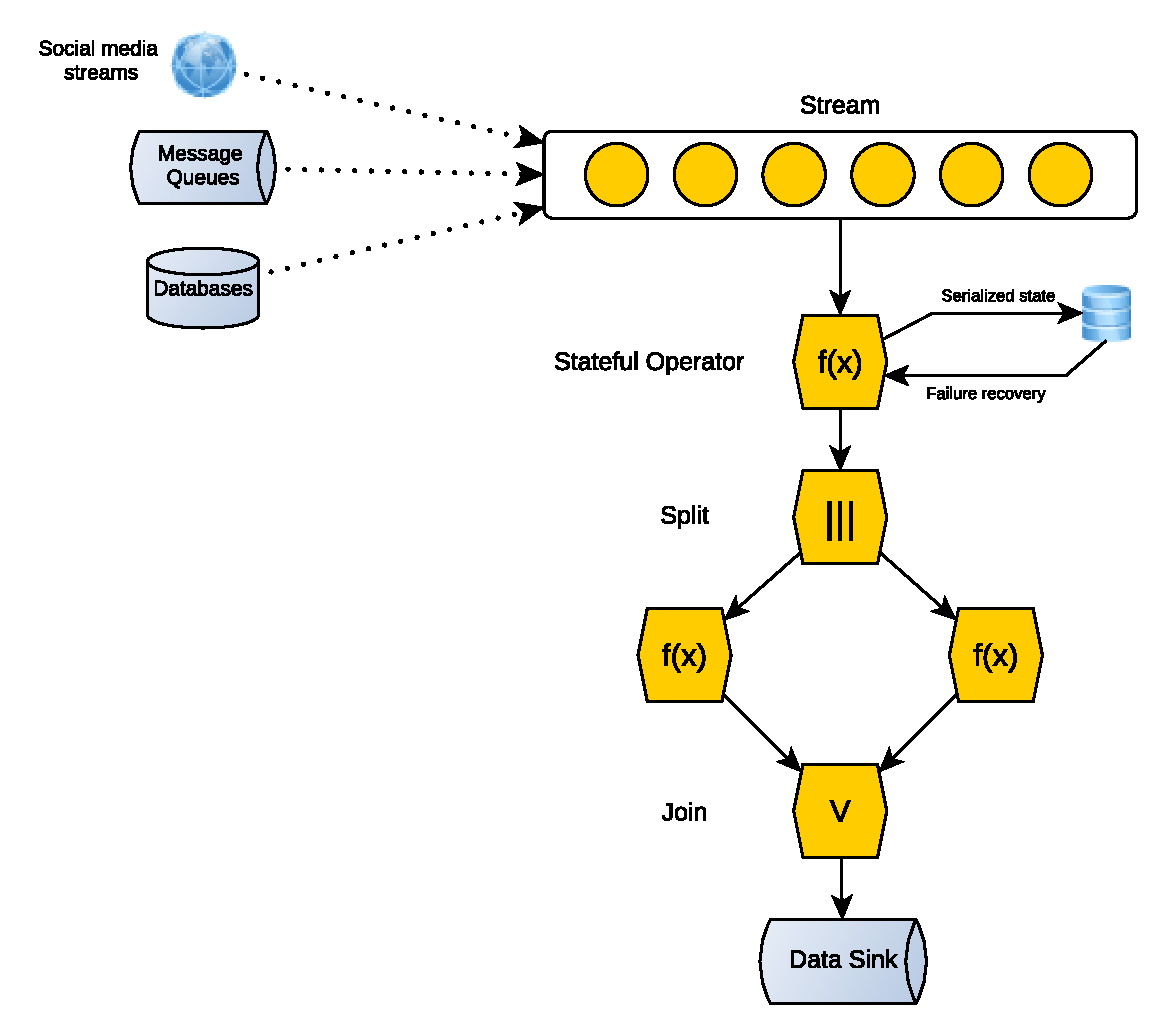
\includegraphics[width=0.45\textwidth,keepaspectratio]{./images/stream-operators.pdf}
		\caption{Stream processing operators.}
	\end{figure}
\end{frame}

\begin{frame}
	\frametitle{Thread Placement}

	\begin{figure}
        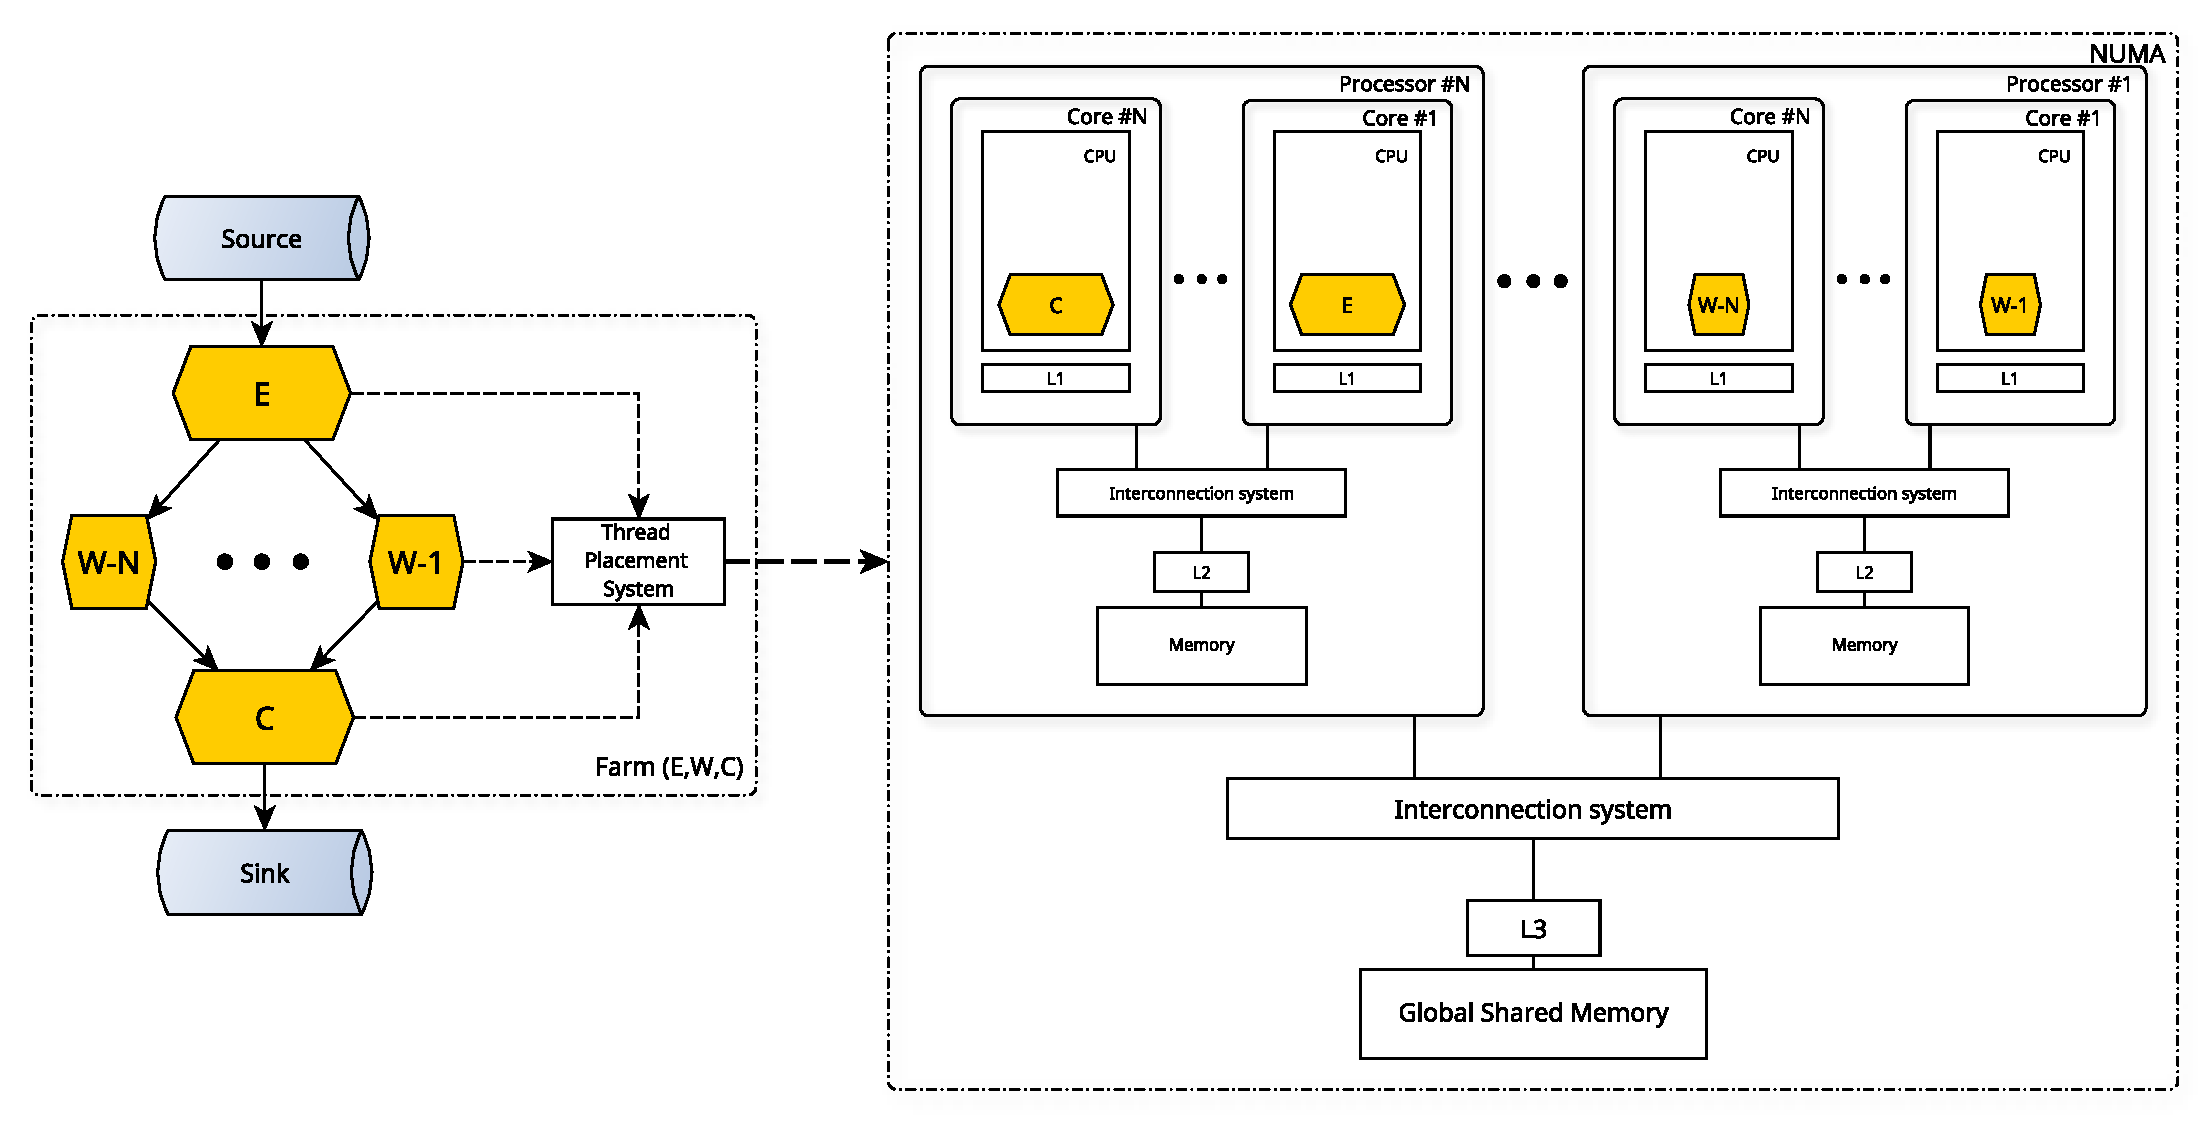
\includegraphics[width=0.7\textwidth,keepaspectratio]{./images/proposed-approach-placement-1.pdf}
		\caption{Stream processing placement 1.}
	\end{figure}
\end{frame}

\begin{frame}
	\frametitle{Thread Placement}

	\begin{figure}
        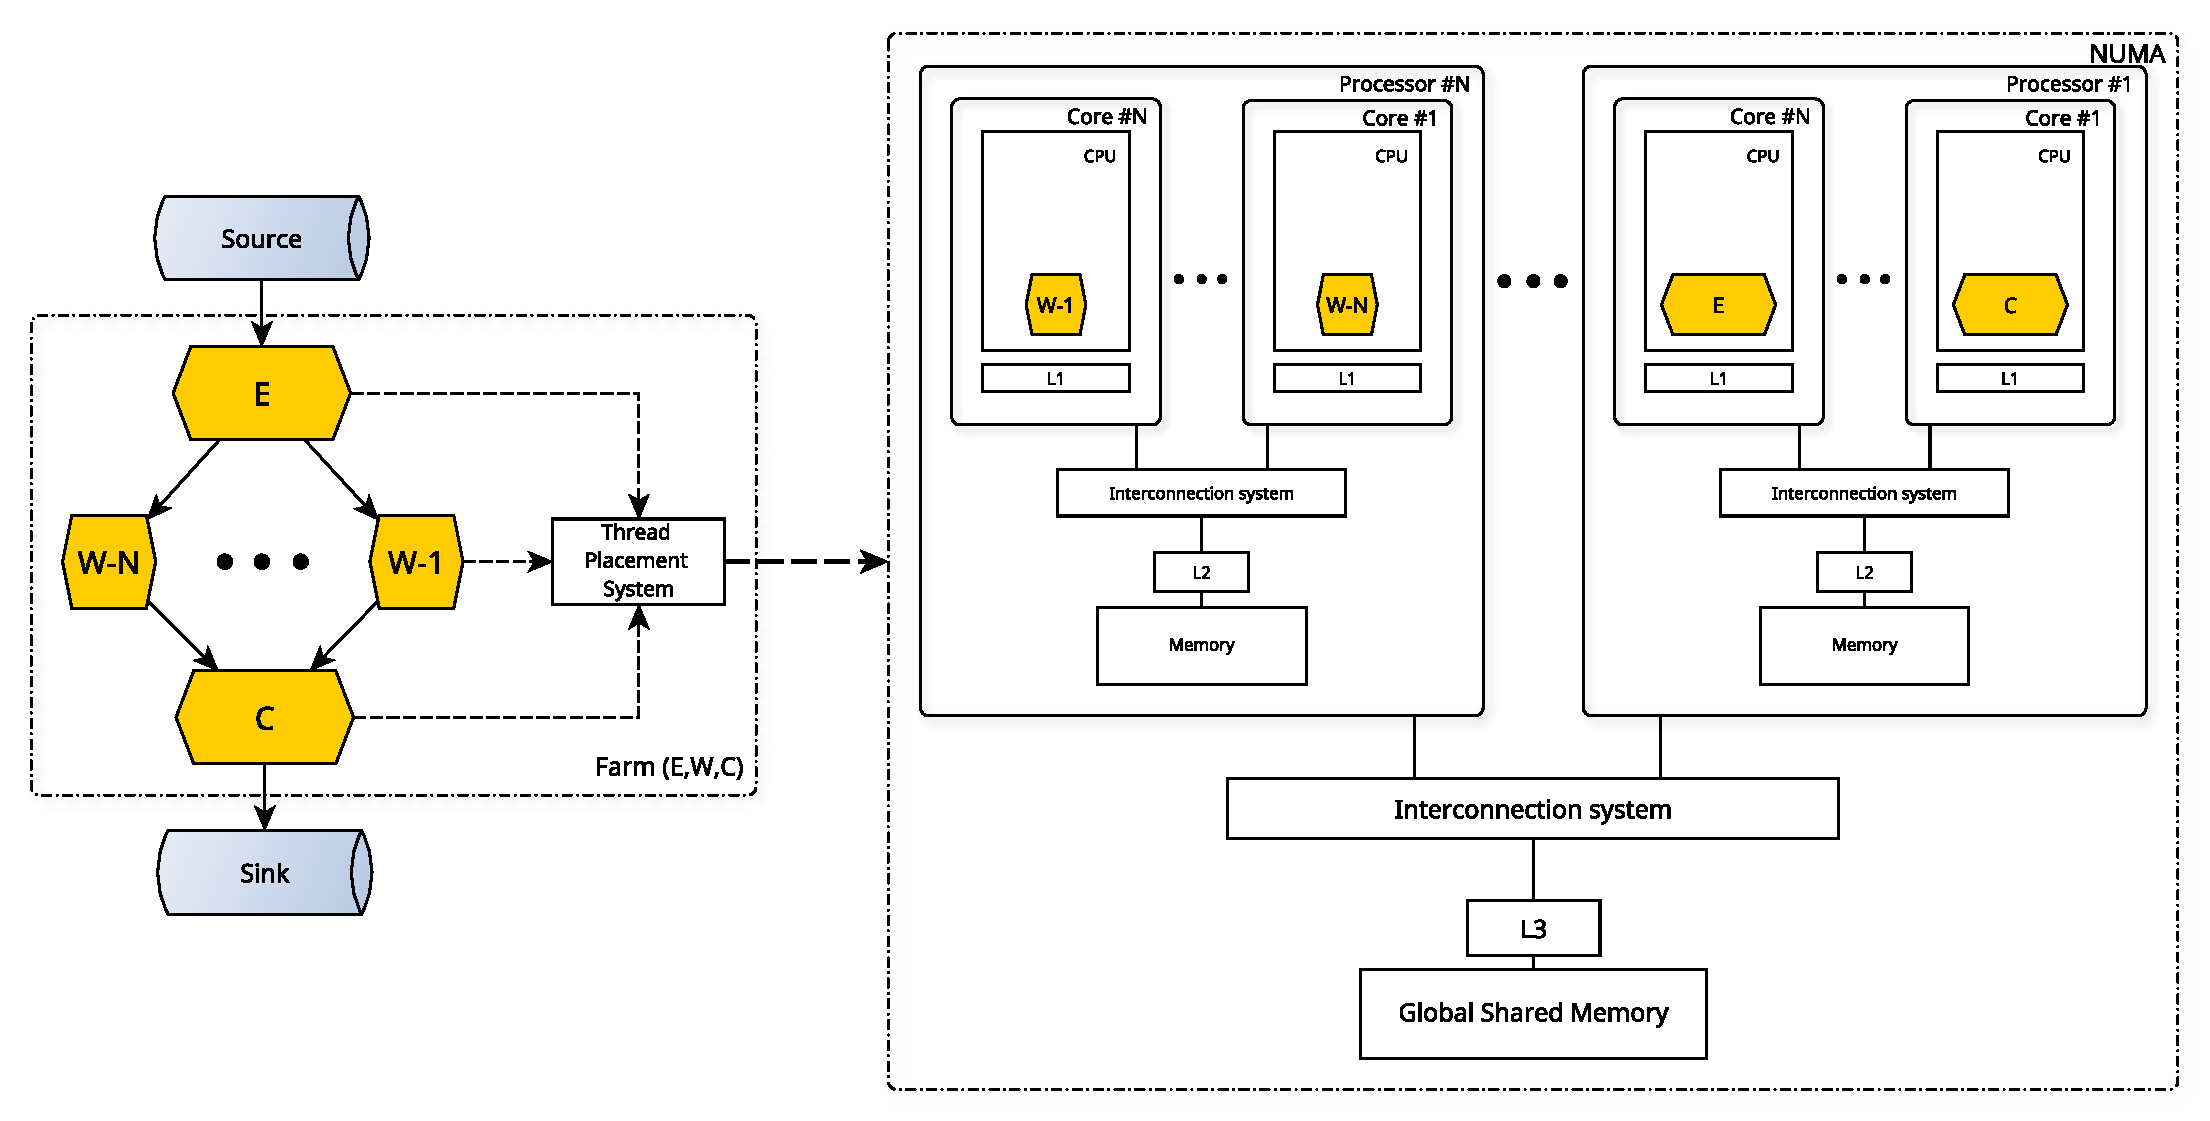
\includegraphics[width=0.7\textwidth,keepaspectratio]{./images/proposed-approach-placement-2.pdf}
		\caption{Stream processing placement 2.}
	\end{figure}
\end{frame}
%---------------------------------------------------------

%---------------------------------------------------------
\section{Perf}

\begin{frame}
	\frametitle{Perf}
    Linux tool to profile CPU performance counters.
    \break
    \break

	\begin{columns}
		\column{0.3\textwidth}
        \begin{block}{\texttt{perf list}}
            \begin{itemize}
                \item cache-misses
                \item instructions
                \item cpu-cycles
                \item L1-dcache-load-misses
                \item LLC-load-misses
                \item branch-misses
                \item bus-cycles
                \item ...
            \end{itemize}
        \end{block}

		\column{0.4\textwidth}
        \begin{block}{Compiling application}
            \begin{itemize}
                \item \texttt{-g}
                \item \texttt{-fno-omit-frame-pointer}
            \end{itemize}
        \end{block}

        \begin{block}{\texttt{perf record -- sleep 10}}
            \begin{itemize}
                \item \texttt{--sample-cpu}
                \item \texttt{--freq 997}
                \item \texttt{--events xxx,yyy}
                \item \texttt{--call-graph dwarf}
            \end{itemize}
        \end{block}

	\end{columns}

\end{frame}

\begin{frame}[fragile]
	\frametitle{Perf Output File}

    {
        \footnotesize
        \begin{lstlisting}
ff-farm 32905 [002] 13134.421023:         19          cache-misses:
        55bb09b38ce5 ff::ff_node::thWorker::svc_init+0x1b (.../ff-farm)
        55bb09b3667d ff::ff_thread::thread_routine+0x3b (.../ff-farm)
        55bb09b341ae ff::proxy_thread_routine+0x23 (.../ff-farm)

ff-farm 32901 [011] 13134.421079:      36331      cache-references:
        7fc88cc40726 __memmove_avx_unaligned_erms+0xb6 (.../libc-2.31.so)
        7fc88ceb58b4 __pthread_attr_setaffinity_new+0x44 (inlined)
        55bb09b36486 ff::init_thread_affinity+0x162 (.../ff-farm)

...
        \end{lstlisting}
    }
\end{frame}

\begin{frame}[fragile]
	\frametitle{Perf Output File}

    \begin{center}
        \begin{tabular}{l l l l l l}
            time & tid & event & counter & cpu & stack \\
            \hline
            13134.421023 & 32905 & cache-misses & 19 & 2 & ff::ff\_node::thWorker::svc\_init\textbar\\
                         &       &              &    &   & ff::ff\_thread::thread\_routine\textbar\\
                         &       &              &    &   & ff::proxy\_thread\_routine \\
            13134.421079 & 32901 & cache-references & 36331 & 11 & \_\_memmove\_avx\_unaligned\_erms\textbar\\
                         &       &              &    &   & \_\_pthread\_attr\_setaffinity\_new\textbar\\
                         &       &              &    &   & ff::init\_thread\_affinity\\
            ...
        \end{tabular}
    \end{center}
\end{frame}
%---------------------------------------------------------

%---------------------------------------------------------
\section{VisPerf}

\begin{frame}
	\frametitle{VisPerf}

    \begin{block}{About}
        \begin{itemize}
            \item Visualize captured PMUs;
            \item Compare different executions of the same application;
            \item See `regions of interest';
        \end{itemize}
    \end{block}

    \begin{block}{Technologies}
        \begin{itemize}
            \item Bash;
            \item Python;
            \item JavaScript;
            \item D3;
            \item React;
        \end{itemize}
    \end{block}
\end{frame}

\begin{frame}
	\frametitle{Demo}

    \url{https://gmap.pucrs.br/claudioscheer/visperf}
\end{frame}

\begin{frame}
	\frametitle{Source code}

    \url{https://github.com/GMAP/visperf}
\end{frame}
%---------------------------------------------------------

%---------------------------------------------------------
\section{Conclusions}

\begin{frame}
	\frametitle{Conclusions}

    \begin{itemize}
        \item It is only a prototype;
        \item Collect more performance metrics;
            \begin{itemize}
                \item Power usage, for example;
            \end{itemize}
        \item Include more evaluation metrics;
        \item Add more visualizations;
        \item Take feedbacks from other developers;
    \end{itemize}
\end{frame}

\begin{frame}
	\frametitle{References}

    \begin{itemize}
        \item \url{https://perf.wiki.kernel.org/index.php/Main_Page}
        \item \url{https://www.brendangregg.com/perf.html}
        \item \url{https://man7.org/linux/man-pages/man1/perf.1.html}
    \end{itemize}
\end{frame}
%---------------------------------------------------------

\end{document}
